\documentclass{article}
\usepackage[preprint]{neurips_2025}

\usepackage[utf8]{inputenc}
\usepackage[T1]{fontenc}
\usepackage{hyperref}
\usepackage{url}
\usepackage{booktabs}
\usepackage{amsfonts, amsmath, amssymb}
\usepackage{nicefrac}
\usepackage{microtype}
\usepackage{xcolor}
\usepackage{graphicx}
\usepackage{subcaption}
\usepackage{natbib}

\title{Direct Factored Gradient Accumulation: Avoiding Dense LM-Head Gradient Materialization in Factored Optimizers}

\author{
  Julio Jose Lena \\
  Independent Researcher \\
  \texttt{juliolena25@gmail.com} \\
  \url{https://orcid.org/0009-0001-0817-6591}
}

\begin{document}

\maketitle

\begin{abstract}
The output projection layer of a language model is a large matrix with shape
$V \times d$, where $V$ is the vocabulary size and $d$ is the hidden dimension.
Conventional training implementations often materialize an equally large dense
gradient buffer for this matrix before the optimizer step. This is wasteful when
the optimizer ultimately consumes only factored row and column statistics, as in
Adafactor-style update rules. I introduce \emph{Direct Factored Gradient
Accumulation} (DF-GA), a direct accumulation method that bypasses dense
LM-head gradient materialization and accumulates the statistics needed by a
factored optimizer from cotangents and hidden states. DF-GA accumulates exact
row and column gradient marginals and uses a martingale-difference model of
logit cotangents to motivate low-dimensional squared-gradient marginals. The
method reduces the gradient-statistics accumulation term from $O(TVd)$ memory
traffic and arithmetic to $O(T(V+d))$, plus the cost of producing logits,
cotangents, and upstream hidden gradients. I implement a prototype in a native
C/Vulkan Ternary SSM training stack on an NVIDIA GeForce RTX 5070. In the
current v12 implementation, the dense $125.25$ MiB \texttt{dlm\_head} buffer is
removed, and internal smoke measurements report throughput rising from
$497$ tok/s to $594$ tok/s in the post-R496 stack with no short-horizon loss
instability. These measurements are preliminary rather than submission-grade:
the paper identifies the mathematical object, the implementation boundary, and
the validation needed before making a full optimizer-equivalence claim.
\end{abstract}

\section{Introduction}

Large-vocabulary language models place unusual pressure on the final output
projection. Given hidden states $h_t \in \mathbb{R}^d$ and logit cotangents
$\delta_t \in \mathbb{R}^V$, the dense LM-head gradient is
\begin{equation}
  G = \sum_{t=1}^T \delta_t h_t^T \in \mathbb{R}^{V \times d}.
\end{equation}
For $V=32{,}064$ and $d=1024$, storing this matrix in FP32 requires
$32064 \cdot 1024 \cdot 4 = 125.25$ MiB. This allocation is modest compared to
the largest training clusters, but it is large in consumer-GPU training stacks
where the model, activations, optimizer state, runtime buffers, and data staging
compete for a 12--24 GB memory budget.

The core observation in this paper is simple: if the downstream optimizer uses
factored row and column statistics, the training loop should not first
materialize a full $V \times d$ gradient matrix merely to reduce it afterward.
Instead, the relevant row and column statistics can be accumulated directly
from the same cotangents and hidden states that would have produced the dense
gradient.

This observation is related to, but distinct from, memory-efficient optimizer
state methods such as Adafactor \citep{shazeer2018adafactor}, SM3
\citep{anil2019sm3}, and gradient-projection approaches such as GaLore
\citep{zhao2024galore}. Those methods reduce optimizer state or update
representation. DF-GA targets the gradient-statistics materialization boundary:
the point at which a dense LM-head gradient buffer is written only to be
compressed into factored statistics later.

It is also related to large-vocabulary loss implementations such as Cut
Cross-Entropy (CCE) \citep{wijmans2024cut}, sampled softmax, and Noise
Contrastive Estimation (NCE). CCE avoids materializing the full logit matrix in
global memory and uses the sparsity of softmax gradients to reduce work. DF-GA
is complementary: it focuses on the optimizer-facing gradient statistics for
the output projection. In its full-vocabulary mathematical form, DF-GA can
consume full-softmax cotangents. The current C/Vulkan prototype, however, is a
sampled/hot-row instantiation inside the project's v12 training stack, and its
empirical claims should be read within that implementation boundary.

The contribution of this draft is therefore threefold:
\begin{enumerate}
  \item a direct formula for row and column gradient marginals of the LM-head
  update without constructing $G$;
  \item a martingale-motivated approximation for row and column
  squared-gradient marginals suitable for factored adaptive optimizers; and
  \item a native C/Vulkan prototype showing that this boundary matters in a
  consumer-GPU training stack.
\end{enumerate}

\section{Related Work}

\paragraph{Factored optimizers.}
Adafactor \citep{shazeer2018adafactor} stores row and column sums of
second-moment estimates for matrix-shaped parameters, then reconstructs a
per-coordinate scale from those low-dimensional factors. SM3
\citep{anil2019sm3} similarly reduces adaptive optimizer memory by maintaining
covering statistics. DF-GA should be understood as a companion mechanism: it
does not merely store factored optimizer state; it avoids materializing the
dense LM-head gradient before those factored statistics are computed.

\paragraph{Projected and low-rank training.}
GaLore \citep{zhao2024galore} reduces memory by projecting gradients into
low-rank subspaces while preserving full-parameter learning. DF-GA is not a
low-rank projection of the whole update matrix. It instead computes row and
column sufficient statistics directly and delegates the per-coordinate scale to
a factored optimizer reconstruction.

\paragraph{Large-vocabulary loss computation.}
Sampled softmax and NCE reduce vocabulary work by optimizing an approximate or
sampled objective \citep{gutmann2010noise, jean2015using}. CCE
\citep{wijmans2024cut} keeps the objective exact while avoiding global-memory
logit materialization. DF-GA addresses a neighboring boundary: avoiding dense
output-gradient materialization when the optimizer update can be expressed
through factored statistics.

\paragraph{IO-aware training kernels.}
FlashAttention \citep{dao2022flashattention} showed that avoiding unnecessary
global-memory traffic can be as important as reducing asymptotic arithmetic.
DF-GA follows the same systems principle for the output-projection gradient:
write the low-dimensional quantities that the optimizer needs, rather than a
large intermediate matrix that will immediately be reduced.

\section{Mathematical Formulation}

Let $W \in \mathbb{R}^{V \times d}$ be the LM-head weight matrix. For position
$t$, the logits and cross-entropy cotangents are
\begin{align}
  z_t &= W h_t, \\
  \delta_t &= p_t - y_t,
\end{align}
where $p_t = \operatorname{softmax}(z_t)$ and $y_t$ is the target distribution.
The dense gradient is
\begin{equation}
  G_{i,j} = \sum_{t=1}^T \delta_{t,i} h_{t,j}.
\end{equation}

DF-GA does not claim to reconstruct the full matrix $G$ exactly from
$O(V+d)$ numbers. Instead, it targets the row and column statistics consumed by
factored optimizers.

\subsection{Exact First-Order Marginals}

Define the row and column gradient marginals
\begin{align}
  r_i &= \sum_{j=1}^d G_{i,j}, \\
  c_j &= \sum_{i=1}^V G_{i,j}.
\end{align}
These can be accumulated directly:
\begin{align}
  r_i &= \sum_{t=1}^T \delta_{t,i} S_h(t),
  \quad S_h(t)=\sum_{j=1}^d h_{t,j}, \\
  c_j &= \sum_{t=1}^T h_{t,j} S_\delta(t),
  \quad S_\delta(t)=\sum_{i=1}^V \delta_{t,i}.
\end{align}
The marginals $r$ and $c$ are exact. They are not the dense gradient matrix.
For an exact full-softmax cross-entropy objective with one-hot targets,
$S_\delta(t)=0$, so the column first-order marginal vanishes. Nonzero column
first-order terms can arise in sampled objectives, weighted objectives, or
straight-through ternary update rules. In a full-softmax Adafactor-style update,
the more central quantity is therefore the factored second moment rather than a
dense first-moment reconstruction.

\subsection{Squared-Gradient Marginals}

Factored adaptive optimizers require row and column summaries of squared
gradients. Let
\begin{align}
  R_i &= \sum_{j=1}^d G_{i,j}^2, \\
  C_j &= \sum_{i=1}^V G_{i,j}^2.
\end{align}
Expanding the row marginal gives
\begin{equation}
  R_i =
  \sum_{t=1}^T \delta_{t,i}^2 \|h_t\|_2^2
  +
  \sum_{t \ne \tau} \delta_{t,i}\delta_{\tau,i}
  \langle h_t, h_\tau\rangle .
\end{equation}
Similarly, the column marginal is
\begin{equation}
  C_j =
  \sum_{t=1}^T h_{t,j}^2 \|\delta_t\|_2^2
  +
  \sum_{t \ne \tau} h_{t,j}h_{\tau,j}
  \langle \delta_t, \delta_\tau\rangle .
\end{equation}

The direct DF-GA estimators drop the cross terms:
\begin{align}
  \widehat{R}_i &= \sum_{t=1}^T \delta_{t,i}^2 \|h_t\|_2^2, \\
  \widehat{C}_j &= \sum_{t=1}^T h_{t,j}^2 \|\delta_t\|_2^2.
\end{align}
This is exact when the cross terms are zero. More generally, it is justified
when the logit cotangents behave approximately as a martingale difference
sequence relative to the training filtration and the hidden-state inner
products do not introduce strong aligned temporal correlations:
\begin{equation}
  \mathbb{E}[\delta_t \mid \mathcal{F}_{t-1}] \approx 0,
  \qquad
  \mathbb{E}[\delta_{t,i}\delta_{\tau,i}
  \langle h_t,h_\tau\rangle] \approx 0
  \quad (t \ne \tau).
\end{equation}
This condition should be treated as an empirical assumption, not as an
unconditional theorem about language model training. A submission-ready version
of this paper should report the measured cross-term residual, temporal
autocorrelation of cotangents, and cosine alignment of the resulting optimizer
updates.

\subsection{Factored Reconstruction}

Given nonnegative row and column squared-gradient marginals, an
Adafactor-style reconstruction can use
\begin{equation}
  \widehat{Q}_{i,j}
  =
  \frac{\widehat{R}_i \widehat{C}_j}
       {\sum_{k=1}^V \widehat{R}_k + \epsilon}.
\end{equation}
The exact normalization convention depends on the optimizer. The key point is
that the dense $V \times d$ squared-gradient table is never stored. DF-GA
therefore changes the materialization boundary, while the optimizer defines how
the factored statistics become a coordinate-wise update scale.

\section{Prototype Implementation}

I implement DF-GA inside the native C/Vulkan Ternary SSM training stack in
\texttt{src/model\_v12/}. The implementation is not a generic PyTorch
autograd drop-in. It is an integrated training-path optimization built around
the existing v12 sampled-softmax and hot-row LM-head update path.

\begin{figure}[h]
  \centering
  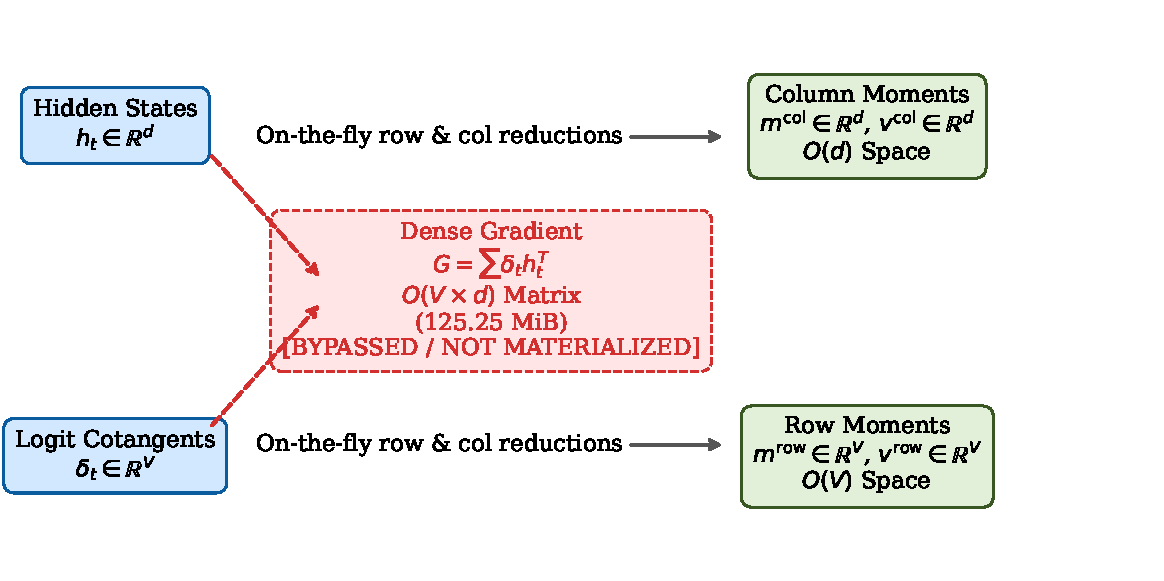
\includegraphics[width=0.8\textwidth]{diagram_dfga.pdf}
  \caption{Data flow of Direct Factored Gradient Accumulation (DF-GA). The dense
  $V \times d$ gradient buffer is bypassed; row and column statistics are
  accumulated directly from cotangents and hidden states.}
  \label{fig:data_flow}
\end{figure}

\paragraph{Training support.}
The current prototype operates on the same candidate-token support used by the
v12 baseline: sampled cotangents and a hot-row update map. Thus, the reported
prototype numbers compare two implementations of the same v12 training path,
not a universal full-vocabulary replacement for dense Adam.

\paragraph{Direct accumulation.}
The Vulkan backend computes losses and cotangents, then the host-side fallback
downloads the valid sampled rows, hidden states after final normalization, and
sample identifiers. The direct accumulator updates row and column gradient
statistics without allocating \texttt{dlm\_head}. This also fixes an important
engineering boundary: only valid sequence rows are copied back from GPU buffers,
avoiding out-of-bounds reads during short or masked batches.

\paragraph{Optimizer integration.}
The factored optimizer consumes the accumulated row and column statistics. In
the current implementation, the LM-head row factor is hot-token indexed and the
column factor is hidden-dimension indexed. This matches the v12 hot/cold update
semantics. It should not be described as updating every vocabulary row unless a
full-vocabulary variant is enabled and validated.

\section{Empirical Status}

The current evidence is promising but not yet complete enough for a strong
conference submission. Table~\ref{tab:status} summarizes the project-local
measurements available at the time of this draft.

\begin{table}[h]
  \centering
  \caption{Current v12 prototype evidence. The throughput and residency numbers
  are post-R496 stack measurements, not a DF-GA-only ablation.}
  \label{tab:status}
  \begin{tabular}{p{0.25\linewidth}p{0.25\linewidth}p{0.40\linewidth}}
    \toprule
    Quantity & Observed value & Claim boundary \\
    \midrule
    Removed dense buffer & $125.25$ MiB & Direct \texttt{dlm\_head} allocation removed \\
    Training throughput & $497 \rightarrow 594$ tok/s & Post-R496 stack smoke, not isolated DF-GA \\
    Steady residency & $530.79 \rightarrow 365.09$ MB & Post-R496 stack smoke \\
    First-order dense audit & $\le 1.14\times 10^{-12}$ max absolute error & Synthetic dense audit; exact row/column marginals \\
    Cross-term residual & $0.084$--$0.123$ in martingale-like controls; $\approx 0.997$ in correlated control & Synthetic diagnostic, not a trainer-speed result \\
    Loss stability & not established & Current default-stack smoke reached NaN at step 1; excluded from the DF-GA claim \\
    \bottomrule
  \end{tabular}
\end{table}

To close the most important mathematical gap in this draft, I added a
repository-local dense audit at
\texttt{scripts/research/paper7\_dfga\_dense\_audit.py}. The audit materializes
$G=\Delta^\top H$ only for measurement on controlled toy shapes, then compares
the dense marginals against the direct streaming statistics. With
$V=256$, $d=128$, and $T\in\{64,128,256,512\}$, first-order row and column
marginals match to floating-point precision in sampled-softmax and Gaussian
martingale-like controls. The squared-marginal residual remains below the
$0.35$ diagnostic budget in those controls, but rises to approximately $0.997$
in a deliberately correlated negative control. This is the right failure mode:
the audit supports the exact first-order claim and makes the second-moment
claim conditional on a measured cross-term residual.

The strongest presently defensible empirical statement is therefore narrower:
removing the dense \texttt{dlm\_head} buffer saves $125.25$ MiB, and the dense
audit verifies the exact first-order statistic contract while exposing the
second-order residual that must be priced. The stronger claims, such as
``DF-GA alone gives a $19.5\%$ speedup'', ``identical convergence'', or
``short-horizon training stability'', require additional validation:
\begin{enumerate}
  \item a production dense-gradient audit that materializes $G$ only for
  measurement and compares exact row/column marginals, squared marginals, and
  update vectors on real v12 batches;
  \item a DF-GA-only ablation against the immediately preceding v12 baseline;
  \item multi-seed loss and perplexity curves on at least one real text corpus;
  \item full-vocabulary and sampled/hot-row variants reported separately; and
  \item profiling that separates LM-head gradient-statistics accumulation from
  logit computation, upstream hidden-gradient computation, and optimizer update.
\end{enumerate}

\section{Limitations}

\paragraph{The martingale condition is empirical.}
The cotangent sequence $\delta_t$ is not guaranteed to be a martingale
difference sequence during training. Early training, repeated text, small
corpora, curriculum structure, and overfitting can produce correlated residuals.
DF-GA therefore needs a cross-term residual diagnostic rather than a purely
verbal appeal to martingale theory.

\paragraph{First-order marginals are not dense gradients.}
The row and column first-order quantities are exact marginals of $G$, but they
do not determine $G$. Any first-moment update reconstructed from them is a
factored update rule, not dense Adam. This is acceptable if the optimizer is
defined around those statistics, but it must be evaluated as an optimizer
choice.

\paragraph{Current implementation is sampled/hot-row.}
The v12 prototype uses sampled cotangents and hot-token row factors. That is a
valid implementation target, but it is not the same as a full-vocabulary
full-softmax implementation. A publishable version should clearly present both
the general formula and the exact production instantiation.

\paragraph{The current figures are not enough.}
Aggregate throughput and loss-smoke numbers are useful engineering evidence,
but paper-grade evidence needs reproducible plots generated from raw logs,
multiple seeds, and clear separation from other R496 optimizations.

\section{Conclusion}

DF-GA is a promising systems-and-optimization mechanism for language-model
training stacks that use factored optimizer statistics. Its central value is not
that a dense LM-head gradient can be magically reconstructed from $O(V+d)$
numbers; it cannot. The value is that many factored optimizers do not need the
dense matrix to be materialized in the first place. Row and column marginals can
be accumulated directly, and squared-gradient marginals can be approximated
under a measurable martingale-style residual condition.

The current C/Vulkan prototype demonstrates that this boundary matters on
consumer hardware by removing a $125.25$ MiB gradient buffer, and the dense
audit now verifies the exact first-order statistic contract in controlled
settings. The idea is worth developing into a paper, but the next version
should replace broad equivalence language with explicit optimizer semantics,
isolate DF-GA in ablation, repair or bypass the current default-stack NaN before
using trainer logs, and report the real-batch cross-term diagnostics that
determine when the martingale approximation is valid.

\bibliographystyle{plainnat}
\bibliography{references}

\end{document}
